\documentclass{beamer}
%\documentclass[aspectratio=169]{beamer}

\usepackage[serbianc]{babel}
\usepackage{graphicx}
\usepackage{makeidx}
\usepackage{listings}
\usepackage{adjustbox}

\hypersetup{unicode}
\makeindex
\usefonttheme{professionalfonts}
\usetheme{CambridgeUS}

\title{Основе веб програмирања}
\author{Борисав Живановић (borisavz)}

\begin{document}

    \begin{frame}
        \maketitle
    \end{frame}

    \begin{frame}{Садржај}
        \begin{enumerate}
            \item Основни појмови мрежног програмирања
            \item Клијент-сервер архитектура
            \item Еволуција веб апликација
            \item HTTP протокол
            \item Рад са базом података
            \item Архитектура веб апликације
            \item Аутентификација и ауторизација
        \end{enumerate}
    \end{frame}

    \section{Основни појмови мрежног програмирања}
    \subsection{Packet switching}

    \begin{frame}[allowframebreaks]{Packet switching}
        \begin{itemize}
            \item Потребно је да поруку пошаљемо примаоцу
            \item Директна веза са сваким примаоцем није остварива
            \item Идеја: повезивање пошиљаоца/примаоца у мрежу, дељење комуникационог канала
            \item Решење: \textbf{комутација пакета (packet switching)}
            \begin{itemize}
                \item Поруку изделимо на пакете
                \item Пакетима додамо заглавље (header) са адресом пошиљаоца и примаоца
                \item Систем зна путање до примаоца
                \item Поруку шаљемо пакет по пакет
                \item Само један пакет заузима комуникациони канал
                \item Пакети могу да путују различитим путањама кроз мрежу, да дођу у различитом редоследу до примаоца, или да нестану
            \end{itemize}
        \end{itemize}

        \framebreak

        \begin{figure}
            \centering
            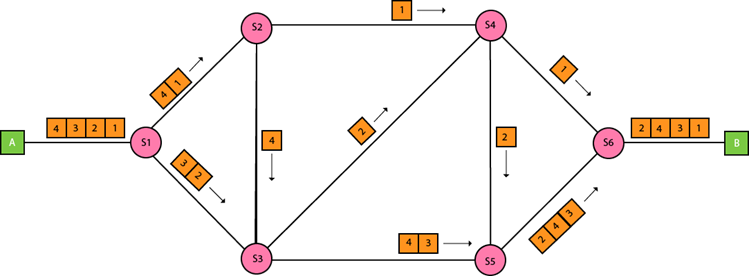
\includegraphics[width=\textwidth,height=0.8\textheight,keepaspectratio]{images/pcsw.png}
            \caption{комутација пакета (packet switching)}
            \label{fig:pcsw}
        \end{figure}
    \end{frame}

    \subsection{IP, DNS}

    \begin{frame}[allowframebreaks]{Internet Protocol}
        \begin{itemize}
            \item Како би комуницирали у мрежи, потребно је да сваки учесник у комуникацији има додељену \textbf{јединствену} адресу
            \item Поруци придружујемо \textbf{заглавље (header)} које садржи:
            \begin{itemize}
                \item Адресу пошиљаоца (source address)
                \item Адресу примаоца (destination address)
                \item Додатна поља (верзија IP протокола, flags, TTL, checksum, ...)
            \end{itemize}
            \item Захваљујући овом заглављу систем зна коме да проследи поруку
            \item У одговори су адресе пошиљаоца и примаоца \textbf{замењене}!
        \end{itemize}

        \framebreak

        \begin{figure}
            \centering
            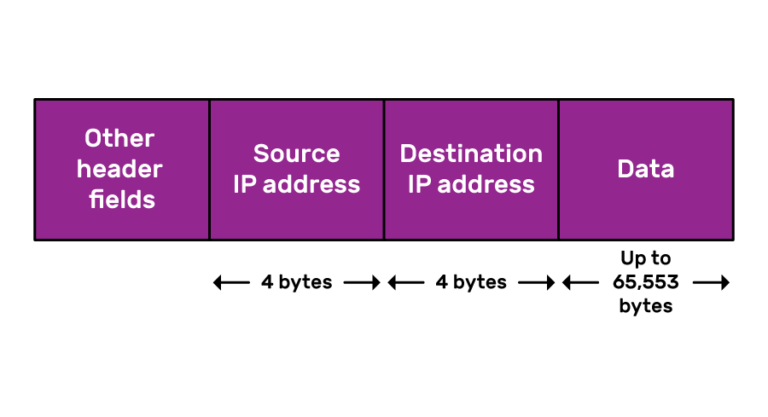
\includegraphics[width=\textwidth,height=\textheight,keepaspectratio]{images/ip.png}
            \caption{упрошћена структура IP пакета}
            \label{fig:ip}
        \end{figure}
    \end{frame}

    \begin{frame}[allowframebreaks]{DNS}
        \begin{itemize}
            \item Проблем: све више сервера на мрежи
            \item Није практично памтити сваку адресу у бројчаном облику
            \item Идеја: систем за придруживање имена, сличан телефонском именику
            \item Решење: \textbf{DNS (Domain Name System)}
            \begin{itemize}
                \item IP адреси додељујемо симболичко име (домен)
                \item Домени су хијерархијски (структура стабла)
                \item DNS је одговоран за одређени део хијерархије
                \item Као одговор враћа IP адресу или адресу одговорног DNS сервера
                \item Морамо знати IP адресу DNS сервера!
            \end{itemize}
        \end{itemize}

        \framebreak

        \begin{figure}
            \centering
            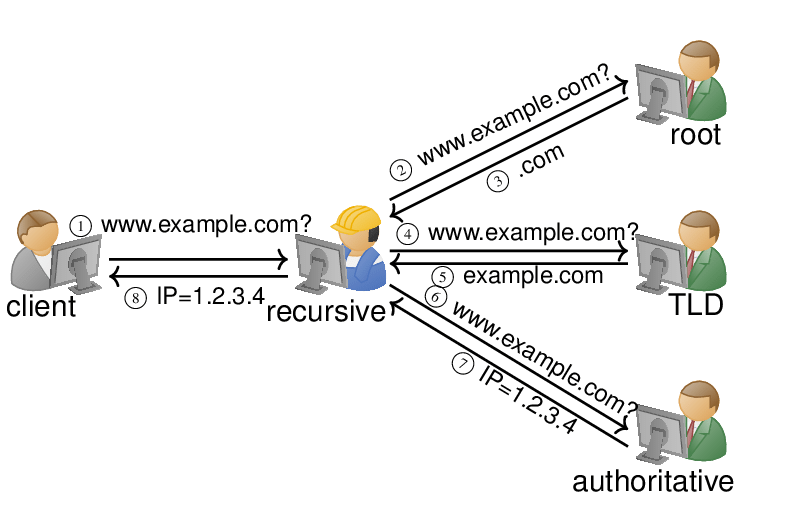
\includegraphics[width=\textwidth,height=0.7\textheight,keepaspectratio]{images/dns.png}
            \caption{DNS упит}
            \label{fig:dns}
        \end{figure}
    \end{frame}
    
    \subsection{TCP, UDP}
    
    \begin{frame}[allowframebreaks]{Transmission Control Protocol}
        \begin{itemize}
            \item Решили смо проблем адресирања уређаја на мрежи...
            \item ...али нисмо проблеме редоследа пристиглих пакета и нестајања пакета
            \item Додатни проблем: шта ако имамо више мрежних апликација на истом рачунару, како да проследимо поруку одговарајућој апликацији?
        \end{itemize}
        
        \framebreak
        
        \begin{itemize}
            \item Решење: \textbf{TCP (Transmission Control Protocol)}
            \begin{itemize}
                \item Додајемо додатно заглавље на нашу поруку
                \item Заглавље садржи source и destination port (слично адреси пошиљаоца и примаоца, али се односи на апликацију), sequence number (редослед поруке)
                \item Уколико пакет нестане, шаље се поново
                \item Оперативни систем осигурава да само једна апликација користи одређени порт
            \end{itemize}
        \end{itemize}
        
        \framebreak
        
        \begin{figure}
            \centering
            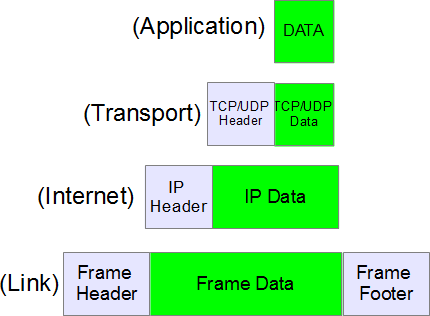
\includegraphics[width=\textwidth,height=0.7\textheight,keepaspectratio]{images/enc.png}
            \caption{енкапсулација пакета}
            \label{fig:tcp_enc}
        \end{figure}
        
        \framebreak
        
        \begin{figure}
            \centering
            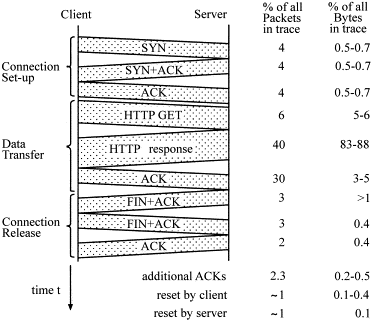
\includegraphics[width=\textwidth,height=0.7\textheight,keepaspectratio]{images/tcp_http.png}
            \caption{Ток TCP комуникације}
            \label{fig:tcp_flow}
        \end{figure}
    \end{frame}
    
    \begin{frame}[allowframebreaks]{User Datagram Protocol}
        \begin{itemize}
            \item Успостављање конекције траје одређено време
            \item За поруке које стају у један пакет, можемо користити једноставнији \textbf{UDP (User Datagram Protocol)}
            \item Задржавамо адресирање апликација, али губимо гаранцију испоруке
            \item DNS користи UDP
            \item Омогућава изградњу протокола који имају гаранције испоруке
            \begin{itemize}
                \item пример: HTTP3/QUIC
            \end{itemize}
        \end{itemize}
    
        \framebreak
        
        \begin{figure}
            \centering
            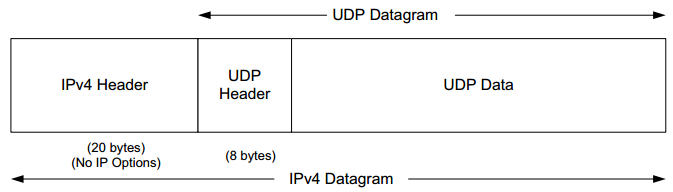
\includegraphics[width=\textwidth,height=\textheight,keepaspectratio]{images/udp_enc.png}
            \caption{енкапсулација пакета}
            \label{fig:udp_enc}
        \end{figure}
        
        \framebreak
        
        \begin{figure}
            \centering
            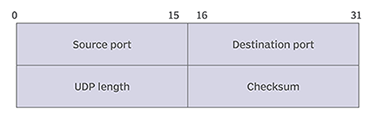
\includegraphics[width=\textwidth,height=\textheight,keepaspectratio]{images/udp_header.png}
            \caption{Садржај заглавља}
            \label{fig:udp_header}
        \end{figure}
    \end{frame}
    
    \section{Клијент-сервер архитектура}
    
    \begin{frame}{Однос између чворова}
        \begin{itemize}
            \item До сада смо говорили искључиво о чворовима који учествују у комуникацији
            \item Видели смо да један чвор започиње комуникацију, а други даје одговор
            \item У раду уочавамо две врсте односа између чворова:
            \begin{itemize}
                \item \textbf{peer-to-peer}: обе стране су подједнако важне у комуникацији
                \item \textbf{client-server}: клијент се обраћа серверу за податке или обављање акције
            \end{itemize}
        \end{itemize}
    \end{frame}
    
    \begin{frame}[allowframebreaks]{Клијент-сервер архитектура}
        \begin{itemize}
            \item Модел настао још раних дана рачунарства
            \item Рачунари су били велики и скупи
            \item Било је потребно омогућити дељење ресурса између више корисника
            \item Клијенти су били далеко једноставнији, главна намена је била слање команде и испис резултата
            \item Данас је овај приступ познат као \textbf{thin-client}
        \end{itemize}
        
        \framebreak
        
        \begin{figure}
            \centering
            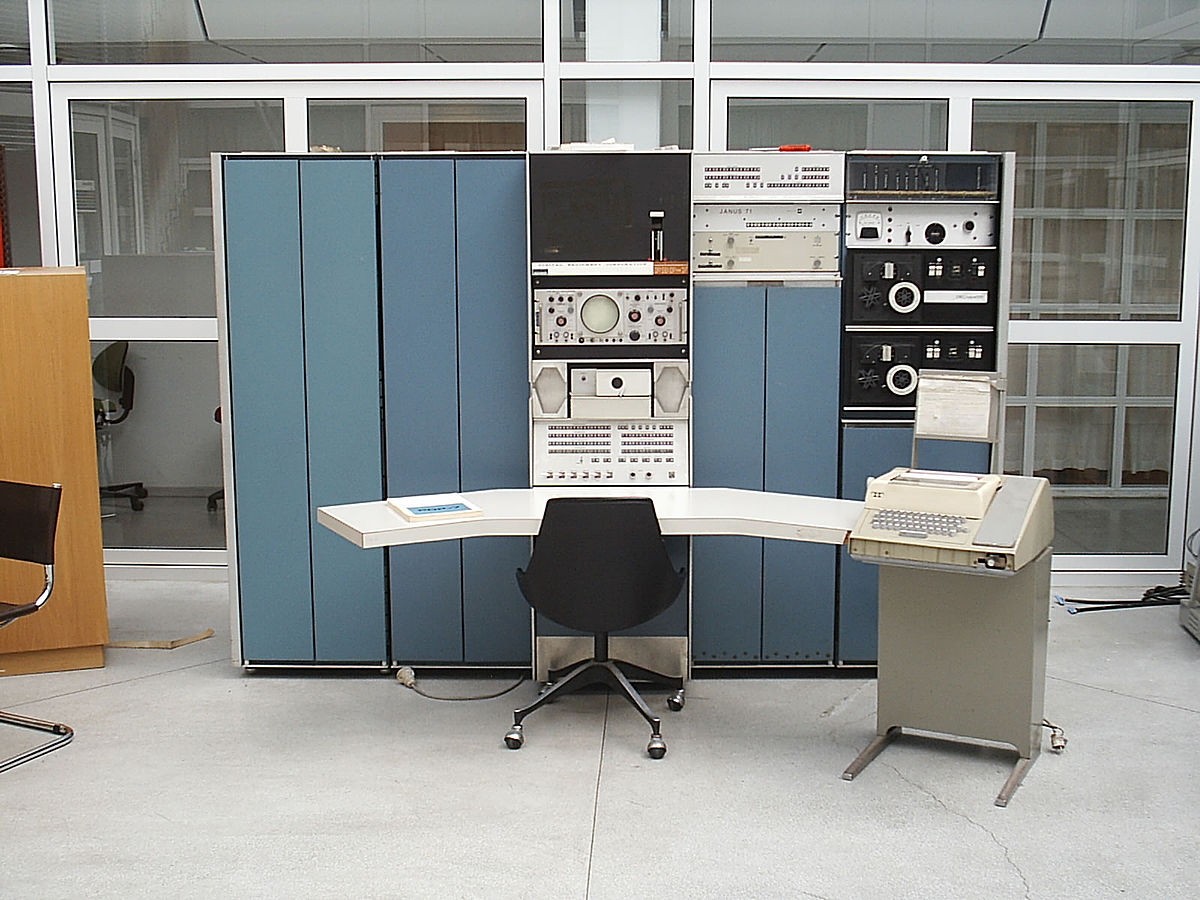
\includegraphics[width=\textwidth,height=0.7\textheight,keepaspectratio]{images/pdp7.jpeg}
            \caption{PDP-7 (рачунар)}
            \label{fig:mainframe}
        \end{figure}
        
        \framebreak
        
        \begin{figure}
            \centering
            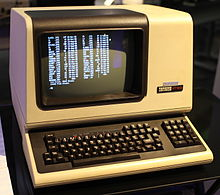
\includegraphics[width=\textwidth,height=0.7\textheight,keepaspectratio]{images/DEC_VT100_terminal.jpg}
            \caption{DEC VT100 (терминал)}
            \label{fig:terminal}
        \end{figure}
        
        \framebreak
        
        \begin{itemize}
            \item Кроз године, рачунарска моћ је расла
            \item Ово је довело до појаве \textbf{PC (Personal Computer)}
            \begin{itemize}
                \item користи се непосредно
                \item без конукурентних корисничких сесија
            \end{itemize}
            \item Потреба за централним сервером и даље није потпуно избачена, али је могућа далеко већа интерактивност
            \item Данас је овај приступ познат као \textbf{thick-client}
            \begin{itemize}
                \item пример: Google Docs
            \end{itemize}
        \end{itemize}
    \end{frame}
    
    \section{Еволуција веб апликација}
    
    \begin{frame}[allowframebreaks]{Еволуција веб апликација}
        \begin{itemize}
            \item \textbf{World Wide Web (WWW)} је изумео Тим Бернерс-Ли у CERN-у
            \item Оригинална замисао је била систем за дељење докумената
            \item Језик докумената: \textbf{HTML (HyperText Markup Language)}
            \item Протокол за комуникацију: \textbf{HTTP (HyperText Transfer Protocol)}
            \item Иницијално садржај је био статички (могуће је прегледање искључиво предефинисаних докумената)
            \item Убрзо су уочени недостаци и настала је потреба за динамичким садржајем
        \end{itemize}
        
        \framebreak
        
        \begin{itemize}
            \item Идеја: чувати садржај у бази података и на основу њега динамички генерисати HTML документе
            \item Постоје два решења:
            \begin{itemize}
                \item \textbf{server-side render}: HTML документ генеришемо користећи шаблон и вредности из базе података
                \item \textbf{client-side render}: са сервера учитавамо основни HTML и JavaScript код, након тога размењујемо JSON објекте
            \end{itemize}
        \end{itemize}
        
        \framebreak
        
        \begin{figure}
            \centering
            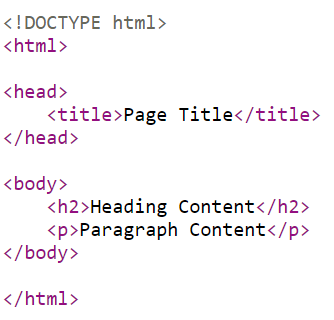
\includegraphics[width=\textwidth,height=0.7\textheight,keepaspectratio]{images/html.png}
            \caption{HTML документ}
            \label{fig:html}
        \end{figure}
        
        \framebreak
        
        \begin{figure}
            \centering
            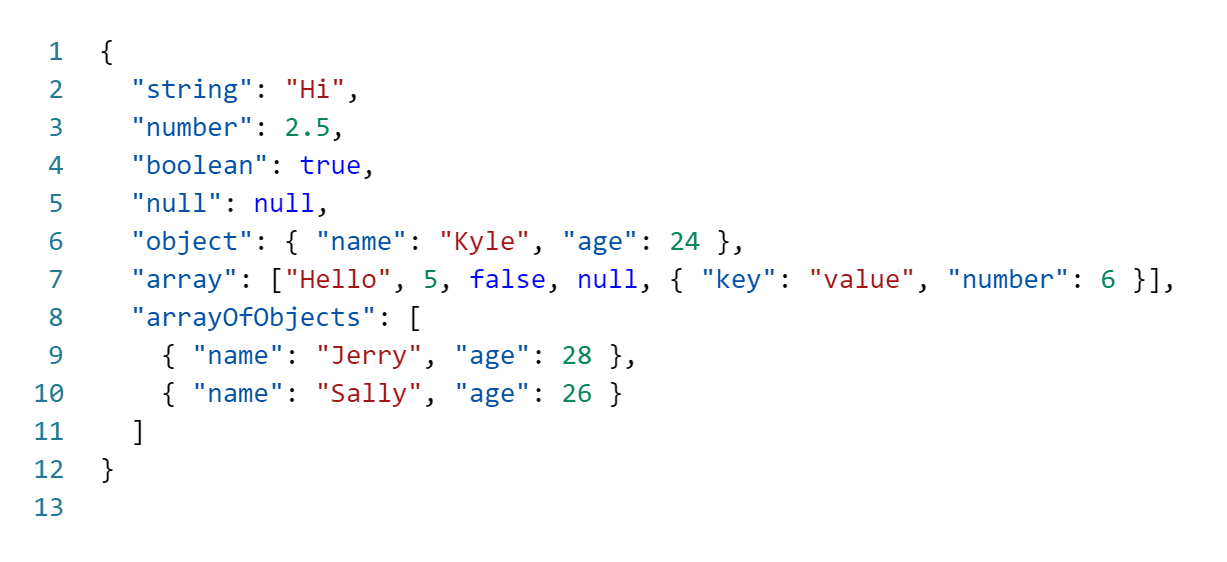
\includegraphics[width=\textwidth,height=0.7\textheight,keepaspectratio]{images/json.png}
            \caption{JSON објекат}
            \label{fig:json}
        \end{figure}
    \end{frame}
    
    \section{HTTP протокол}
    
    \begin{frame}{HTTP протокол}
        \begin{itemize}
            \item Текстуални протокол (поруке једноставно могу да читају и људи)
            \item Користи TCP (гаранција испоруке је неопходна како би протокол успешно функционисао!)
            \item Подразумевани порт: 80 (HTTP), 443 (HTTPS)
            \item Stateless протокол
            \begin{itemize}
                \item неопходно је придружити додатне информације уз сваки захтев како би пратили корисничку сесију
                \item обично преко header-a
            \end{itemize}
            \item Путања означава \textbf{ресурс} у систему
            \begin{itemize}
                \item додатни атрибути кроз \textbf{query params}
            \end{itemize}
            \item Метода означава \textbf{акцију} коју желимо да извршимо над ресурсом
            \item Статусни код означава да ли је акција успешно изврешна, и ако није, разлог
        \end{itemize}
    \end{frame}
    
    \begin{frame}[allowframebreaks]{Request-response}
        \begin{figure}
            \centering
            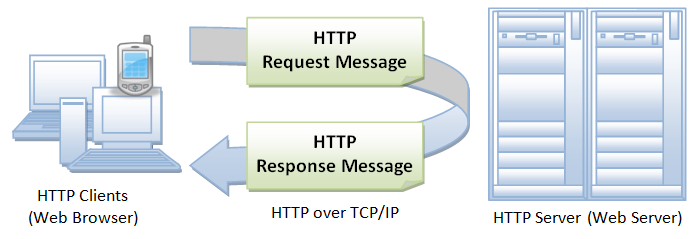
\includegraphics[width=\textwidth,height=\textheight,keepaspectratio]{images/reqres.png}
            \caption{Request-response модел}
            \label{fig:reqres}
        \end{figure}
        
        \framebreak
        
        \begin{figure}
            \centering
            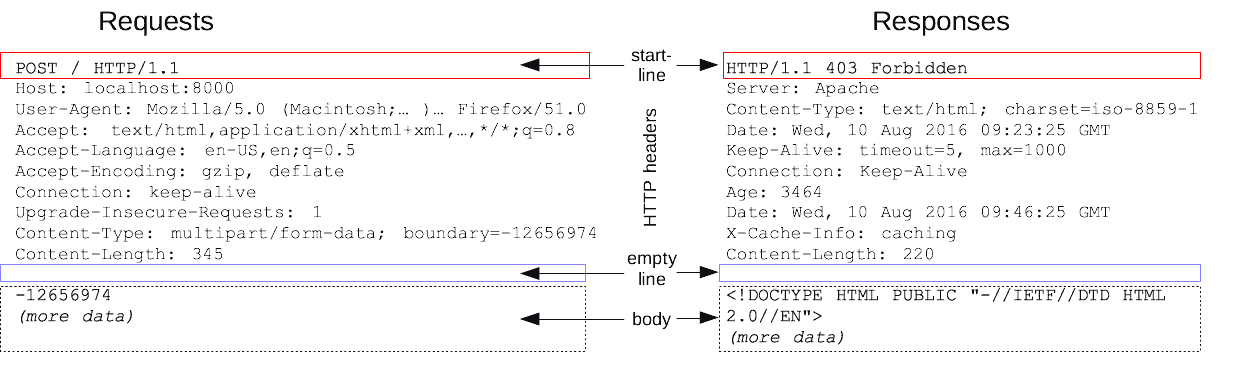
\includegraphics[width=\textwidth,height=\textheight,keepaspectratio]{images/httpmsgstructure.png}
            \caption{Садржај \textbf{request} и \textbf{response} порука}
            \label{fig:reqrescont}
        \end{figure}
        
        \framebreak
        
        \begin{itemize}
            \item Формирамо HTTP захтев (string)
            \item Извршавамо DNS упит како би добили IP адресу сервера
            \begin{itemize}
                \item могуће је и кеширање DNS одговора на клијентској страни
            \end{itemize}
            \item Успостављамо TCP конекцију са сервером (подразумевани или наведени порт)
            \item Захтев шаљемо издељен у пакете
            \item Чекамо одговор
            \begin{itemize}
                \item клијенти обично постављају timeout
            \end{itemize}
            \item Затварамо TCP конекцију
            \begin{itemize}
                \item потенцијално уско грло уколико у кратком временском периоду шаљемо више захтева
                \item исправљено у наредним верзијама протокола
            \end{itemize}
        \end{itemize}
        
        \framebreak
        
        \begin{figure}
            \centering
            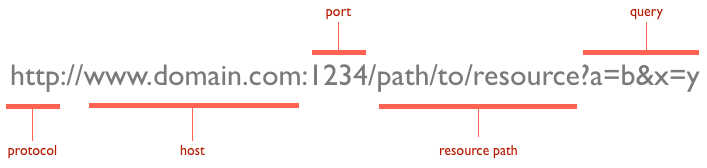
\includegraphics[width=\textwidth,height=\textheight,keepaspectratio]{images/url.png}
            \caption{URL}
            \label{fig:url}
        \end{figure}
    \end{frame}
    
    \begin{frame}{HTTP методе}
        \begin{itemize}
            \item \textbf{GET}: добављање ресурса из система
            \item \textbf{PUT}: измена постојећег ресрса у целости
            \item \textbf{POST}: додавање новог ресурса у систем
            \item \textbf{PATCH}: измена дела постојећег ресурса
            \item \textbf{DELETE}: брисање ресурса из система
        \end{itemize}
    \end{frame}
    
    \begin{frame}{Status codes}
        \begin{itemize}
            \item \textbf{1xx}: информациони одговор
            \begin{itemize}
                \item 100 Continue, 101 Switching Protocols, 103 Early Hints, ...
            \end{itemize}
            \item \textbf{2xx}: успешан одговор
            \begin{itemize}
                \item 200 OK, 201 Created, 202 Accepted, ...
            \end{itemize}
            \item \textbf{3xx}: редирекција
            \begin{itemize}
                \item 301 Moved Permanently, 302 Found, ...
            \end{itemize}
            \item \textbf{4xx}: грешка клијента
            \begin{itemize}
                \item 400 Bad Request, 401 Unauthorized, 403 Forbidden, 404 Not Found, 405 Method Not Allowed, 415 Unsupported Media Type, 422 Unprocessable Entity, ...
            \end{itemize}
            \item \textbf{5xx}: грешка сервера
            \begin{itemize}
                \item 500 Internal Server Error, 501 Not Implemented, 502 Bad Gateway, 503 Service Unavailable, 505 HTTP Version Not Supported, ...
            \end{itemize}
        \end{itemize}
    \end{frame}

    \section{Архитектура веб апликације}
    
    \begin{frame}[allowframebreaks]{Архитектура веб апликације}
        \begin{itemize}
            \item Потребно је да омогућимо комуникацију преко HTTP
            \item И да комуницирамо са базом како би извршавали упите
            \item Једну акцију може да чини више упита ка бази
            \item Потребно је запис у бази представити структуром података у жељеном програмском језику
            \item ...и то су, у суштини, компоненте веб апликације
        \end{itemize}
        
        \framebreak
        
        \begin{figure}
            \centering
            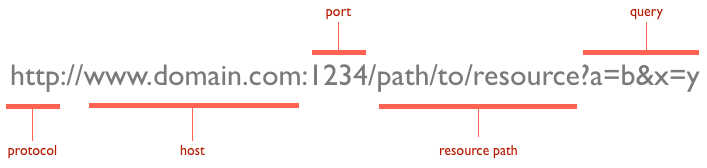
\includegraphics[width=\textwidth,height=\textheight,keepaspectratio]{images/url.png}
            \caption{шематски приказ архитектуре}
            \label{fig:url}
        \end{figure}
    \end{frame}
    
    \subsection{Controller}
    
    \begin{frame}{Controller}
        \begin{itemize}
            \item Садржај HTTP захтева претвара у структуру података
            \item Позива методу из сервисног слоја
            \item Резултат добијен позивом сервисног слоја претвара у HTTP одговор
            \item Може да садржи логику за ауторизацију
            \item Упозорење: грешка коју шаљемо клијенту не сме да открива интерне детаље
        \end{itemize}
    \end{frame}
    
    \begin{frame}[fragile]{Пример имплементације: Go/Gorilla Mux}
        \begin{adjustbox}{width=\textwidth,height=\textheight,keepaspectratio}
            \begin{lstlisting}[language=go]
func (c *AuthController) VerifyRegistration(w http.ResponseWriter, req *http.Request) {
    ctx, span := c.tracer.Start(req.Context(), "AuthController.VerifyRegistration")
    defer span.End()

    verificationId := mux.Vars(req)["verificationId"]

    appErr := c.authService.VerifyRegistration(ctx, verificationId)
    if appErr != nil {
        span.SetStatus(codes.Error, appErr.Error())
        http.Error(w, appErr.Message, appErr.Code)
        return
    }
}
            \end{lstlisting}
        \end{adjustbox}
    \end{frame}
    
    \begin{frame}[fragile]{Пример имплементације: Java/Spring}
        \begin{adjustbox}{width=\textwidth,height=\textheight,keepaspectratio}
            \begin{lstlisting}[language=java]
@PostMapping("/{postId}/comments")
@IsLoggedIn
public long addPostComment(
        @PathVariable long postId,
        @RequestBody @Valid CreateCommentDTO createCommentDTO
) {
    return postService.addPostComment(postId, createCommentDTO);
}

            \end{lstlisting}
        \end{adjustbox}
    \end{frame}
    
    \subsection{Service}
    
    \begin{frame}{Service}
        \begin{itemize}
            \item Садржи пословну логику апликације
            \item Једна сервисна метода се састоји из позива једне или више метода из repository
            \item Уколико база података подржава трансакције, сервисна метода је граница трансакције
            \begin{itemize}
                \item \textbf{commit} уколико је акција успешна
                \item \textbf{rollback} уколико је акција неуспешна
            \end{itemize}
            \item Садржи комплетне провере права приступа
            \begin{itemize}
                \item чест шаблон је да извршимо упит који проверава да ли корисник има право приступа (рецимо, чланство на пројекту), и у зависности од резултата извршимо акцију
            \end{itemize}
        \end{itemize}
    \end{frame}
    
    \begin{frame}[fragile]{Пример имплементације: Go/Gorilla Mux}
        \begin{adjustbox}{width=\textwidth,height=\textheight,keepaspectratio}
            \begin{lstlisting}[language=go]
func (s *AuthService) VerifyRegistration(ctx context.Context, verificationId string) *app_errors.AppError {
    serviceCtx, span := s.tracer.Start(ctx, "AuthService.VerifyRegistration")
    defer span.End()

    username, err := s.authRepository.GetVerification(serviceCtx, verificationId)
    if err != nil {
        span.SetStatus(codes.Error, err.Error())
        return &app_errors.AppError{500, ""}
    }

    user, err := s.authRepository.GetUser(serviceCtx, username)

    user.Enabled = true

    err = s.authRepository.SaveUser(serviceCtx, user)
    if err != nil {
        span.SetStatus(codes.Error, err.Error())
        return &app_errors.AppError{500, ""}
    }

    err = s.authRepository.DeleteVerification(serviceCtx, verificationId)
    if err != nil {
        span.SetStatus(codes.Error, err.Error())
        return &app_errors.AppError{500, ""}
    }

    return nil
}
            \end{lstlisting}
        \end{adjustbox}
    \end{frame}
    
    \begin{frame}[fragile]{Пример имплементације: Java/Spring}
        \begin{adjustbox}{width=\textwidth,height=\textheight,keepaspectratio}
            \begin{lstlisting}[language=java]
@Transactional
public void downvotePost(long postId) {
    Post post = postRepository.getById(postId);
    User user = userRepository.getById(authUser().getId());

    if(post.getCommunity().isUserBanned(user))
        throw new NotAllowedToParticipateException();

    reactionRepository.deletePostReactionByUser(authUser().getId(), postId);

    Reaction reaction = new Reaction();

    reaction.setMadeBy(user);
    reaction.setPost(post);
    reaction.setType(ReactionType.DOWNVOTE);

    reactionRepository.save(reaction);
}
            \end{lstlisting}
        \end{adjustbox}
    \end{frame}
    
    \subsection{Repository}
    
    \begin{frame}{Repository}
        \begin{itemize}
            \item Једна метода представља један упит над базом података
            \item Параметре прослеђује у упит
            \begin{itemize}
                \item подсетник: потребно је да се одбранимо од injection напада!
            \end{itemize}
            \item Резултат упита претвара у одговарајуће структуре података
            \begin{itemize}
                \item \textbf{entity} уколико враћамо записе из базе неизмењене
                \item \textbf{DTO} уколико упит садржи комплекснија пресликавања (пример: генерисање извештаја)
            \end{itemize}
            \item У зависности од коришћене базе података/библиотеке, логику за конверзију резултата упита морамо ручно да имплементирамо, или библиотека то чини аутоматски
        \end{itemize}
    \end{frame}
    
    \begin{frame}[fragile]{Пример имплементације: Go/Gorilla Mux}
        \begin{adjustbox}{width=\textwidth,height=\textheight,keepaspectratio}
            \begin{lstlisting}[language=go]
func (r *ConsulAuthRepository) DeleteUser(ctx context.Context, username string) error {
    _, span := r.tracer.Start(ctx, "ConsulAuthRepository.DeleteUser")
    defer span.End()

    kv := r.cli.KV()

    userKey, err := r.constructKey("user/%s/", username)
    if err != nil {
        span.SetStatus(codes.Error, err.Error())
        return err
    }

    _, err = kv.Delete(userKey, nil)
    if err != nil {
        span.SetStatus(codes.Error, err.Error())
        return err
    }

    return nil
}
            \end{lstlisting}
        \end{adjustbox}
    \end{frame}
    
    \begin{frame}[fragile]{Пример имплементације: Java/Spring}
        \begin{adjustbox}{width=\textwidth,height=\textheight,keepaspectratio}
            \begin{lstlisting}[language=java]
@Modifying
@Query(value = "" +
        " DELETE FROM reaction" +
        " WHERE made_by_id = ?1" +
        " AND post_id = ?2",
        nativeQuery = true)
void deletePostReactionByUser(long userId, long postId);
            \end{lstlisting}
        \end{adjustbox}
    \end{frame}
    
    \subsection{Entity}
    
    \begin{frame}{Entity}
        \begin{itemize}
            \item Представља записе у бази података
            \begin{itemize}
                \item додатно: везе ка другим ентитетима
            \end{itemize}
            \item Омогућује објектно-релационо мапирање
            \item Може да садржи бизнис логику
            \begin{itemize}
                \item тема активне дебате
            \end{itemize}
        \end{itemize}
    \end{frame}
    
    \begin{frame}[fragile]{Пример имплементације: Go/Gorilla Mux}
        \begin{adjustbox}{width=\textwidth,height=\textheight,keepaspectratio}
            \begin{lstlisting}[language=go]
type User struct {
    Username     string `json:"username"`
    PasswordHash string `json:"passwordHash"`
    Email        string `json:"email"`
    Role         string `json:"role"`
    Enabled      bool   `json:"enabled"`
}
            \end{lstlisting}
        \end{adjustbox}
    \end{frame}
    
    \begin{frame}[fragile]{Пример имплементације: Java/Spring}
        \begin{adjustbox}{width=0.65\textwidth,height=\textheight,keepaspectratio}
            \begin{lstlisting}[language=java]
@Getter
@Setter
@Entity
@EqualsAndHashCode(of = "id")
@SQLDelete(sql = "UPDATE post SET deleted = true WHERE id=?")
@Where(clause = "deleted=false")
public class Post {

    @Id
    @GeneratedValue
    private long id;

    private String title;
    private String text;
    private LocalDate creationDate;

    private long imageId;

    @ManyToOne(fetch = FetchType.EAGER)
    private User postedBy;

    @ManyToOne(fetch = FetchType.EAGER)
    private Community community;

    @ManyToOne(fetch = FetchType.EAGER)
    private Flair flair;

    private boolean deleted;
}
            \end{lstlisting}
        \end{adjustbox}
    \end{frame}
    
    \subsection{Data Transfer Object}
    
    \begin{frame}{Data Transfer Object (DTO)}
        \begin{itemize}
            \item Проблем: ентитети потенцијално нису погодни за слање клијенту
            \item Идеја: применити принцип енкапсулације, трансформација одговора у погодан формат
            \item Ова компонента је опциона, и често није неопходна
            \item Могуће је и комбиновање уз entity
        \end{itemize}
    \end{frame}
    
    \begin{frame}[fragile]{Пример имплементације: Go/Gorilla Mux}
        \begin{adjustbox}{width=\textwidth,height=\textheight,keepaspectratio}
            \begin{lstlisting}[language=go]
type RegisterUser struct {
    Username     string `json:"username" validate:"required"`
    Password     string `json:"password" validate:"required,password"`
    Email        string `json:"email" validate:"required,email"`
    FirstName    string `json:"firstName" validate:"required"`
    LastName     string `json:"lastName" validate:"required"`
    Town         string `json:"town" validate:"required"`
    Gender       string `json:"gender" validate:"required"`
    CaptchaToken string `json:"captchaToken" validate:"required"`
}
            \end{lstlisting}
        \end{adjustbox}
    \end{frame}
    
    \begin{frame}[fragile]{Пример имплементације: Java/Spring}
        \begin{adjustbox}{width=0.7\textwidth,height=\textheight,keepaspectratio}
            \begin{lstlisting}[language=java]
@Getter
@Setter
public class CommentDTO {

    private long id;

    private String text;
    private LocalDate timestamp;
    private long postId;

    private List<CommentDTO> replies;
    private UserDTO writtenBy;

    private ReactionType reaction;
    private int karma;
}
            \end{lstlisting}
        \end{adjustbox}
    \end{frame}
    
    \subsection{Middleware}
    
    \begin{frame}{Middleware}
        \begin{itemize}
            \item Често желимо да централизујемо логику која је потребна пре/после извршавања (већине или свих) метода из контролера
            \begin{itemize}
                \item валидација токена за ауторизацију
                \item праћење информација за logging/tracing
            \end{itemize}
            \item Математички посматрано, одговара композицији функције
            \item У програмским језицима који имају first-class функције (пример: JavaScript, Go) се имплементира као композиција функција
            \item Уколико то није подржано, имплементира се механизмом који то опонаша (пример: Java/Aspect Oriented Programming)
            \item Пресрећемо захтев, прослеђујемо га даље или прекидамо ланац
        \end{itemize}
    \end{frame}
    
    \begin{frame}[fragile]{Пример имплементације: Go/Gorilla Mux}
        \begin{adjustbox}{width=\textwidth,height=0.7\textheight,keepaspectratio}
            \begin{lstlisting}[language=go]
func ExtractJWTUserMiddleware(next http.Handler) http.Handler {
    return http.HandlerFunc(func(w http.ResponseWriter, r *http.Request) {
        if authHeader, ok := r.Header["Authorization"]; ok {
            tokenString := authHeader[0]

            token, err := jwt.Parse(tokenString, func(token *jwt.Token) (interface{}, error) {
                return []byte(os.Getenv("SECRET_KEY")), nil
            })

            if claims, ok := token.Claims.(jwt.MapClaims); ok && token.Valid {
                authUser := model.AuthUser{
                    Username: claims["username"].(string),
                    Role:     claims["role"].(string),
                    Exp:      time.UnixMilli(int64(claims["exp"].(float64))),
                }

                authCtx := context.WithValue(r.Context(), "authUser", authUser)

                next.ServeHTTP(w, r.WithContext(authCtx))
            } else {
                http.Error(w, "Invalid token", 401)
            }
        } else {
            next.ServeHTTP(w, r.WithContext(newCtx))
        }
    })
}
            \end{lstlisting}
        \end{adjustbox}
    \end{frame}
    
    \begin{frame}[fragile]{Пример имплементације: Java/Spring}
        \begin{adjustbox}{width=\textwidth,height=0.7\textheight,keepaspectratio}
            \begin{lstlisting}[language=java]
@Override
protected void doFilterInternal(HttpServletRequest request,
                                HttpServletResponse response,
                                FilterChain chain)
        throws ServletException, IOException {
    final String token = request.getHeader(HttpHeaders.AUTHORIZATION);
    if (isEmpty(token)) {
        chain.doFilter(request, response);
        return;
    }

    if (!jwtTokenUtil.validate(token)) {
        response.setStatus(HttpServletResponse.SC_UNAUTHORIZED);
        return;
    }

    User user = userRepository.findByUsername(jwtTokenUtil.getUsername(token)).orElse(null);
    UserDetails userDetails = user == null ? null : new AuthUserDetails(user);

    UsernamePasswordAuthenticationToken authentication = new UsernamePasswordAuthenticationToken(
            userDetails,
            null,
            userDetails == null ? List.of() : userDetails.getAuthorities()
    );

    SecurityContextHolder.getContext().setAuthentication(authentication);
    chain.doFilter(request, response);
}
            \end{lstlisting}
        \end{adjustbox}
    \end{frame}
    
    \section{Аутентификација и ауторизација}
    \subsection{Индирекција}
    
    \begin{frame}[allowframebreaks]{Индирекција}
        \begin{itemize}
            \item Било који проблем у рачунарству може бити решен још једним нивоом индирекције, осим наравно проблема превише индирекција (David J. Wheeler)
            \item Индирекција омогућава имплементацију контроле приступа
            \item Извршавање \textbf{акције} мора да одобри \textbf{посредник} који дефинише правила приступа
            \item Механизам присутан на свим нивоима апстракције
            \begin{itemize}
                \item енкапсулација у ООП, x86 protection rings, системски позиви, изолација процеса, \textbf{бизнис логика}
            \end{itemize}
        \end{itemize}
        
        \framebreak
        
        \begin{figure}
            \centering
            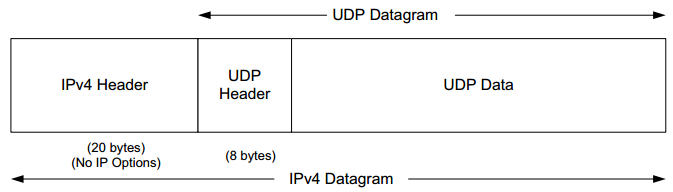
\includegraphics[width=\textwidth,height=\textheight,keepaspectratio]{images/udp_enc.png}
            \caption{шематски приказ индирекције}
            \label{fig:udp_enc}
        \end{figure}
    \end{frame}
    
    \subsection{Основни појмови}
    
    \begin{frame}{Основни појмови}
        \begin{itemize}
            \item \textbf{Идентификација}: процес приписивања идентитета човеку или другом рачунару
            \begin{itemize}
                \item регистрација корисничког налога
            \end{itemize}
            \item \textbf{Аутентификација}: процес провере идентитета
            \begin{itemize}
                \item пријављивање на кориснички налог
            \end{itemize}
            \item \textbf{Ауторизација}: утврђивање права која корисник има над ресурсима у систему
            \begin{itemize}
                \item провере права приступа у апликацији (middleware/controller/service)
            \end{itemize}
        \end{itemize}
    \end{frame}
    
    \subsection{RBAC}
    
    \begin{frame}{Role Based Access Control: концепт}
        \begin{itemize}
            \item Корисник има улогу, улога има дозволе
            \begin{itemize}
                \item улога одговара радном месту у фирми или типу налога (обичан/администраторски)
                \item дозвола одговара акцији у систему
            \end{itemize}
            \item Улога додељена кориснику се (релативно) ретко мења
            \begin{itemize}
                \item промена радног места
            \end{itemize}
            \item Кроз време, могућа је промена дозвола додељених улогама
        \end{itemize}
    \end{frame}
    
    \begin{frame}{Role Based Access Control: имплементација}
        \begin{itemize}
            \item Уз корисника, у бази података чувамо његову улогу
            \item Дозволе се најчешће не чувају, већ се провере имплементирају ручно у middleware/controller
            \item Улога се чува у \textbf{access token}
        \end{itemize}
    \end{frame}
    
    \subsection{ABAC}
    
    \begin{frame}{Attribute Based Access Control: концепт}
        \begin{itemize}
            \item RBAC је погодан за статичке дозволе, али је веома непогодан за динамичке
            \begin{itemize}
                \item пример: само члан сме да приступи пројекту, преузимање видео игре је дозвољено старијима од 16 година
            \end{itemize}
            \item Функција \begin{math}f(Attr) \rightarrow Bool\end{math} одређује да ли корисник има дозволу да обави акцију
            \item \begin{math}Attr\end{math} се састоји од тренутног стања система
            \begin{itemize}
                \item што значи да \begin{math}f(Attr)\end{math} није детерминистичка функција!
            \end{itemize}
        \end{itemize}
    \end{frame}
    
    \begin{frame}{Attribute Based Access Control: имплементација}
        \begin{itemize}
            \item Уз записе у бази чувамо атрибуте који су потребни за одређивање права приступа
            \item Атрибути могу да представљају везу између корисника и заштићеног ресурса (пример: листа чланова пројекта) или да буду везани директо за заштићени ресурс (пример: старост потребна за преузимање игре)
            \item Провере се обављају у сервисном слоју
            \begin{itemize}
                \item уколико се \begin{math}f(Attr)\end{math} евалуира у \begin{math}False\end{math}, враћамо грешку \textbf{403 Forbidden}
            \end{itemize}
            \item Обично захтева додатни упит над базом података
        \end{itemize}
    \end{frame}
    
    \subsection{Складиштење лозинки}
    
    \begin{frame}[allowframebreaks]{Складиштење лозинки}
        \begin{itemize}
            \item Најједноставнији начин је складиштење лозинке у отвореном тексту
            \begin{itemize}
                \item уколико нападач дође у посед лозинки, може да се несметано пријави у нашу, а вероватно и остале апликације
            \end{itemize}
            \item Нешто боље је складиштење \textit{hash}-a лозинке \begin{math}hash = HashFunc(pass)\end{math}
            \begin{itemize}
                \item исте лозинке имају исти \textit{hash} (\begin{math}HashFunc(pass)\end{math} је детерминистичка функција)
                \item могуће је извести dictionary/brute force напад и тиме компоромитовати исте лозинке
            \end{itemize}
            
            \framebreak
            
            \item Најбоље је складиштење \textit{salted hash}-a лозинке \begin{math}salted\_hash = HashFunc(pass + salt)\end{math}
            \begin{itemize}
                \item \begin{math}salt\end{math} је насумична вредност која се складишти уз лозинку
                \item две исте лозинке ће због тога имати различиту \begin{math}salted\_hash\end{math} вредност, па је dictionary/brute force напад потребно извести одвојено за сваку лозинку
            \end{itemize}
            \item На жалост, и даље има доста апликација које лозинке складиште у отвореном тексту, што нас чини рањивим
            \item Напомена: лозинке не смеју да се шаљу уколико веза није безбедна (HTTPS), јер у супротном могу да буду украдене без обзира на безбедно складиштење!
            
            \framebreak
        
            \begin{figure}
                \centering
                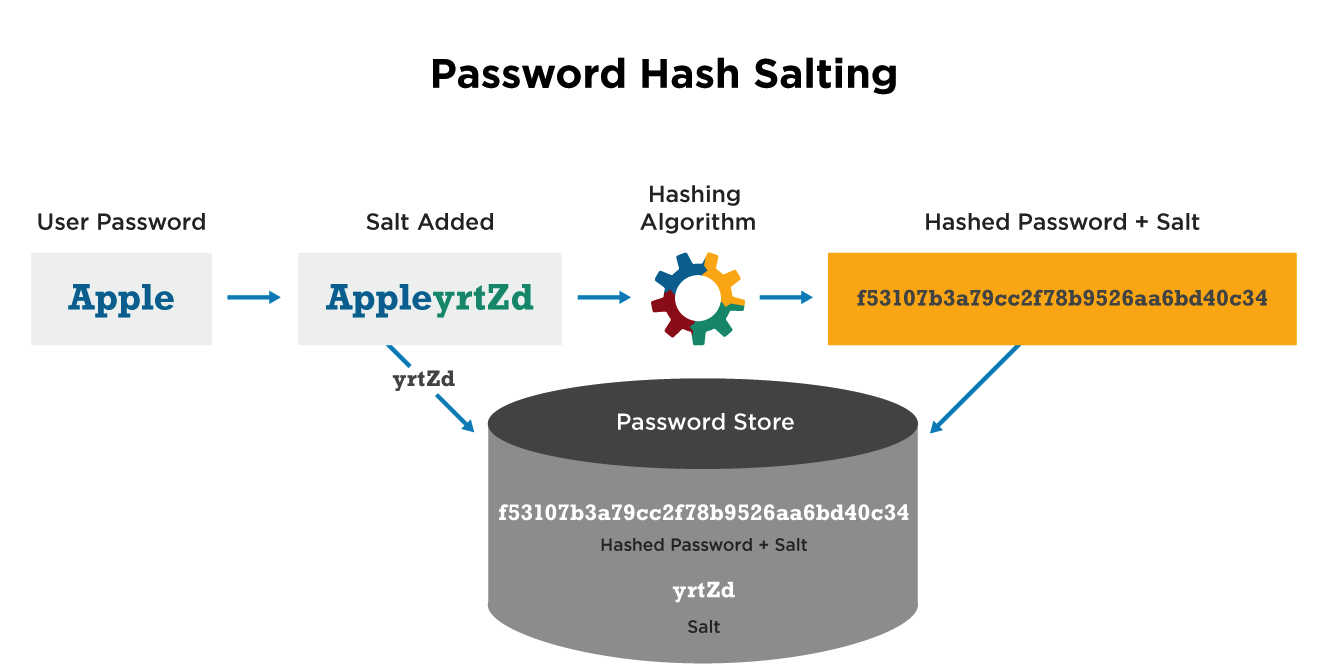
\includegraphics[width=0.9\textwidth,height=\textheight,keepaspectratio]{images/hashsalt.png}
                \caption{шематски приказ \textit{salted hash}-a}
                \label{fig:hashsalt}
            \end{figure}
        \end{itemize}
    \end{frame}
    
    \subsection{Имплементација механизма}
    
    \begin{frame}{Основни ток}
        \begin{itemize}
            \item Креира се кориснички налог
            \begin{itemize}
                \item у зависности од врсте апликације, корисник се самостално региструје или добија готов налог
            \end{itemize}
            \item Корисник се пријављује у апликацију својим креденцијалима (корисничко име и лозинка) и добија access token
            \begin{itemize}
                \item access token садржи ID корисника као и његову улогу
            \end{itemize}
            \item Уз сваки захтев, корисник шаље свој access token
            \begin{itemize}
                \item уколико access token истекне, потребно је да се корисник поново пријави
            \end{itemize}
        \end{itemize}
    \end{frame}
    
    \begin{frame}[allowframebreaks]{OAuth 2.0}
        \begin{itemize}
            \item Проблем: како да омогућимо да друга апликација буде клијент који извршава акције у име корисника?
            \item Једноставно решење: апликацији дајемо креденцијале
            \begin{itemize}
                \item дељење креденцијала никада није добра идеја
                \item апликација би имала сва корисничка права
            \end{itemize}
            \item Боље решење: апликацији дајемо \textit{access token}
            \begin{itemize}
                \item нема дељења креденцијала
                \item токен има ограничена права приступа на неопходан подскуп \begin{math}token\_rights \subseteq user\_rights\end{math}
            \end{itemize}
            \item Ми ћемо да имплементирамо упроштену верзију која не подржава \textit{3rd party} клијенте
            \begin{itemize}
                \item \textbf{Resource Owner Password Credentials Grant} без \textit{refresh token}-a
            \end{itemize}
        \end{itemize}
        
        \framebreak
        
        \begin{figure}
            \centering
            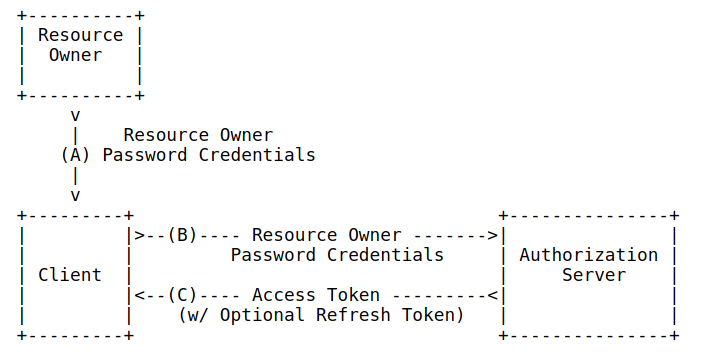
\includegraphics[width=\textwidth,height=\textheight,keepaspectratio]{images/oauth.png}
            \caption{Resource Owner Password Credentials Grant}
            \label{fig:oauth}
        \end{figure}
    \end{frame}
    
    \begin{frame}{Access token}
        \begin{itemize}
            \item Издаје га \textbf{Authorization Server}, шаљемо га у сваком захтеву ка \textbf{Resource Server}
            \item Уколико је токен истекао, или је из другог разлога невалидан, \textbf{Resource Server} одбија наш захтев
            \item Уколико је токен валидан, даља права приступа одређује логика апликације (подсетник: RBAC, ABAC)
            \item Напомена: \textbf{Authorization Server} и \textbf{Resource Server} не морају да буду одвојене апликације, већ одвојени \textit{endpoint}-и у једној апликацији
        \end{itemize}
    \end{frame}
    
    \begin{frame}[allowframebreaks]{JSON Web Token}
        \begin{itemize}
            \item Формат за представљање \textit{access token}-а
            \item \textbf{Header}: Тип токена и алгоритам коришћен за дигитални потпис
            \item \textbf{Payload}: ID корисника, улога, датум док којег важи токен, додатна поља
            \item \textbf{Signature}: Дигитални потпис који апликација проверава како би утврдила да ли је она издала токен
            \item Напомена: Base64 је алгоритам за кодирање, а не енкрипцију!
            \begin{itemize}
                \item односно, свако може да прочита наш токен, те он не би требало да садржи тајне информације
            \end{itemize}
        \end{itemize}
        
        \framebreak
        
        \begin{figure}
            \centering
            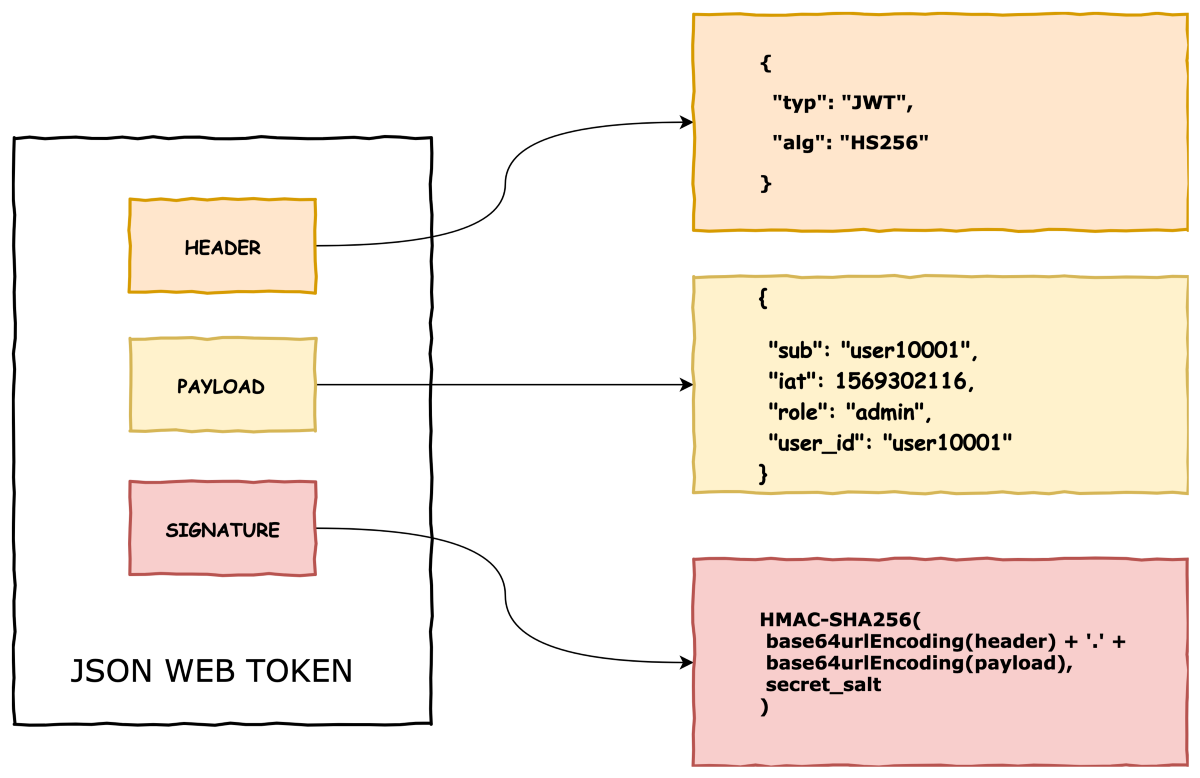
\includegraphics[width=0.9\textwidth,height=0.9\textheight,keepaspectratio]{images/jwt.png}
            \label{fig:jwt}
        \end{figure}
        
        \framebreak
        
        \begin{figure}
            \centering
            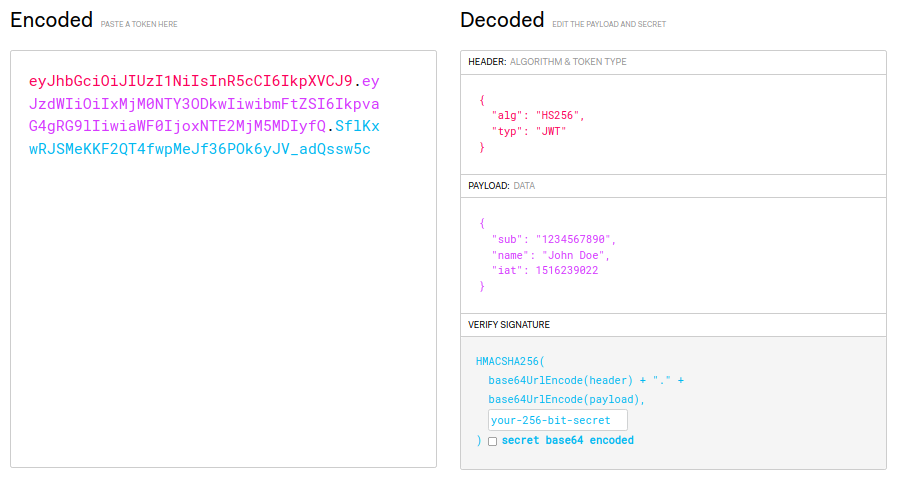
\includegraphics[width=0.9\textwidth,height=0.9\textheight,keepaspectratio]{images/jwt_enc.png}
            \label{fig:jwt_enc}
        \end{figure}
    \end{frame}
    
\end{document}
